\section{Experiment 1: Horizontal and vertical bars}
\label{section:horvertAdaptiveInhibition}

\subsection{Introduction}

% TODO, copy introduction from horvert with stupid inhibition
For this experiment the impact of a neuron layer that encodes a-priori information should be analysed.
% IT sucks, TODO improve

\subsection{Methods}
 % TODO everything copied until "old stuff", look through and adapt
\paragraph{Input data}
29 x 29 black and white images with either horizontal or vertical oriented bars on them were used, as it was more straightforward to express a-priori information. The orientation of the training images was chosen randomly via a uniform distribution. Also the positions of the bars in the images were uniformly distributed. The rest of the image generation process is analogous to experiment 1, except no circular mask was used. Examples of the input data can be seen in Figure \ref{fig:horvertImages}. To show the value of the a-priori information validation images with two bars forming a cross were also generated, seen in Figure \ref{fig:horvertTrainingCrossImage}. When shown to the network in the validation process the prior neurons were given the information that a cross is either in horizontal or vertical orientation.

\begin{figure}
  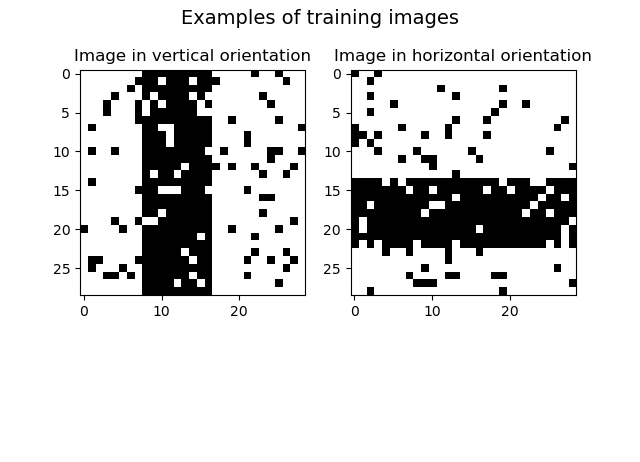
\includegraphics[width=\linewidth]{figures/horvert/horvertTrainingImages.png}
  \caption{Training images generated for experiment 2. One image of each possible orientation at a random position.}
  \label{fig:horvertImages}
\end{figure}

\begin{figure}
  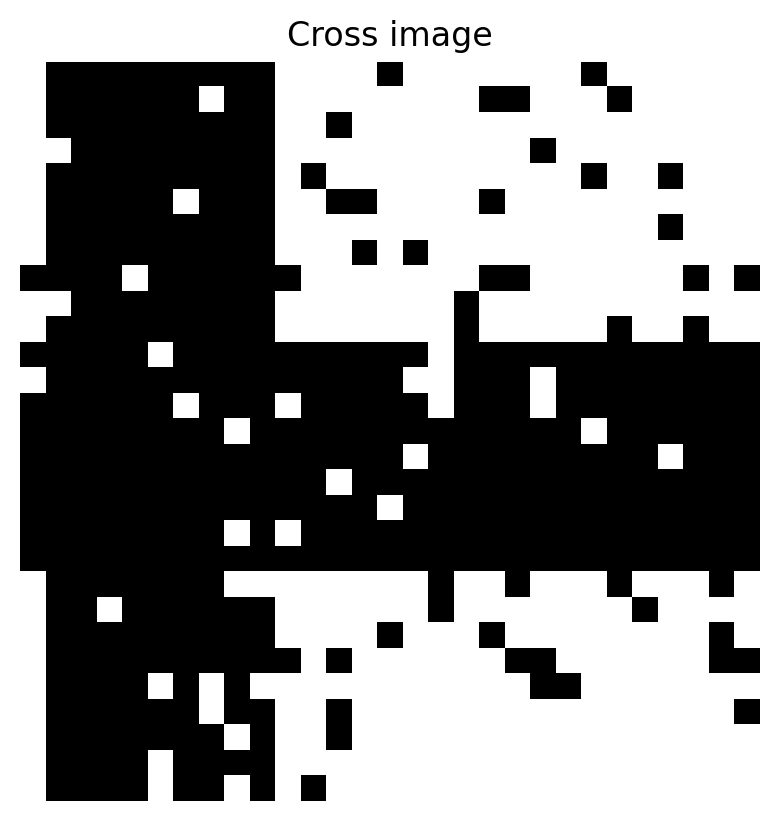
\includegraphics[width=0.6\linewidth]{figures/horvert/horvertTrainingCrossImage.png}
  \caption{Generated cross image which can represent either horizontal or vertical orientation.}
  \label{fig:horvertTrainingCrossImage}
\end{figure}


\paragraph{Network architecture}

This experiment used a expanded version of the network used in experiment 1. An additional layer of prior neurons $z_1,z_2$ was added. Whenever an image was oriented vertically $z_1$ was active and $z_2$ was inactive. For horizontal orientations $z_2$ was active and $z_1$ was inactive. Prior neurons in an active state had a firing frequency of 50 Hz and fired with 0 Hz when inactive.

\paragraph{Neuron model}
The input and output neurons functioned the same way as in the previous experiment. The prior neurons fire according to a poisson process with their firing rate. Each prior neuron $Z_l$ is connected to every output neuron $Y_k$ and thus has weights $w_{kl}$ that were learned by the network. 

\paragraph{Parameters}
As the amount of input neurons and the average number of black pixels in an input image stayed roughly the same in this experiment, the same parameters $c=  20$ and $\lambda = 10^{-3}$ could be used.

%% TODO START
%% this block was copied to Theoretical Background, cut this accordingly
%% Zfactor does not exist, remove!!!
 However as there are only two prior neurons, a way to amplify their produced signals was needed, otherwise their impact on the membrane potential of the output neurons would not be distinctive enough. So the EPSPs $z_l(t)$ were multiplied by the factor $Z_{factor}$. This factor was determined via grid search. The additional prior layer resulted in an expanded version of the membrane potential $u_k(t)$

\begin{equation}
\label{eqn:ukHorvert}
u_k(t) = \sum_{i=1}^n w_{ki} \cdot x_i(t) + \sum_{j=1}^n w_{kj} \cdot Z_{factor} \cdot z_j(t).
\end{equation}

% the old stuff, needed
The firing rate of the output neurons was set to 200 Hz. As there are fewer prior neurons (keine ahung wie viele) to increase the influence of the prior neurons the firing rate of the prior neurons was set to 200 Hz. This change alone did not increase the impact of the prior neurons enough to help the network correctly detect a "cross-bar image" as either horizontal or vertical. It was also tried to increase the parameter $c_{prior}$ for the learning of the prior weights to shift the weight values towards bigger values. This did not increase the values of the weights, they stayed at a maximum of four. Thus the number of prior neurons had to be increased. Via grid search different numbers of prior neurons were tried.
% the old stuff END

\subsection{Results}

The tried parameters were as follows:
\begin{itemize}
  \item $c = c_{prior} = 20$
  \item $\lambda = 10^{-3}$
  \item number of prior neurons $ = 10, 20, 50, 100, 200$
\end{itemize}

For 50, 100 and 200 prior neurons the training process was impaired by the activity of the prior neurons. This arose as some output neurons responding to too large areas, while other prior neurons not responding to any specific areas. For 50 prior neurons four output neurons responded to horizontal bars, while six output neurons responded to vertical bars. This was unexpected and might be due to the stochastic nature of the training image generation. This was not yet analysed further and the validation of the network was performed with 20 prior neurons, as it was the largest amount of prior neurons that resulted in a properly trained network. The results of the training process can be seen in Figures \ref{fig:horvertAdaptiveInhibitionTraining} and \ref{fig:horvertAdaptiveInhibitionpriorWeights}.

\begin{figure}
  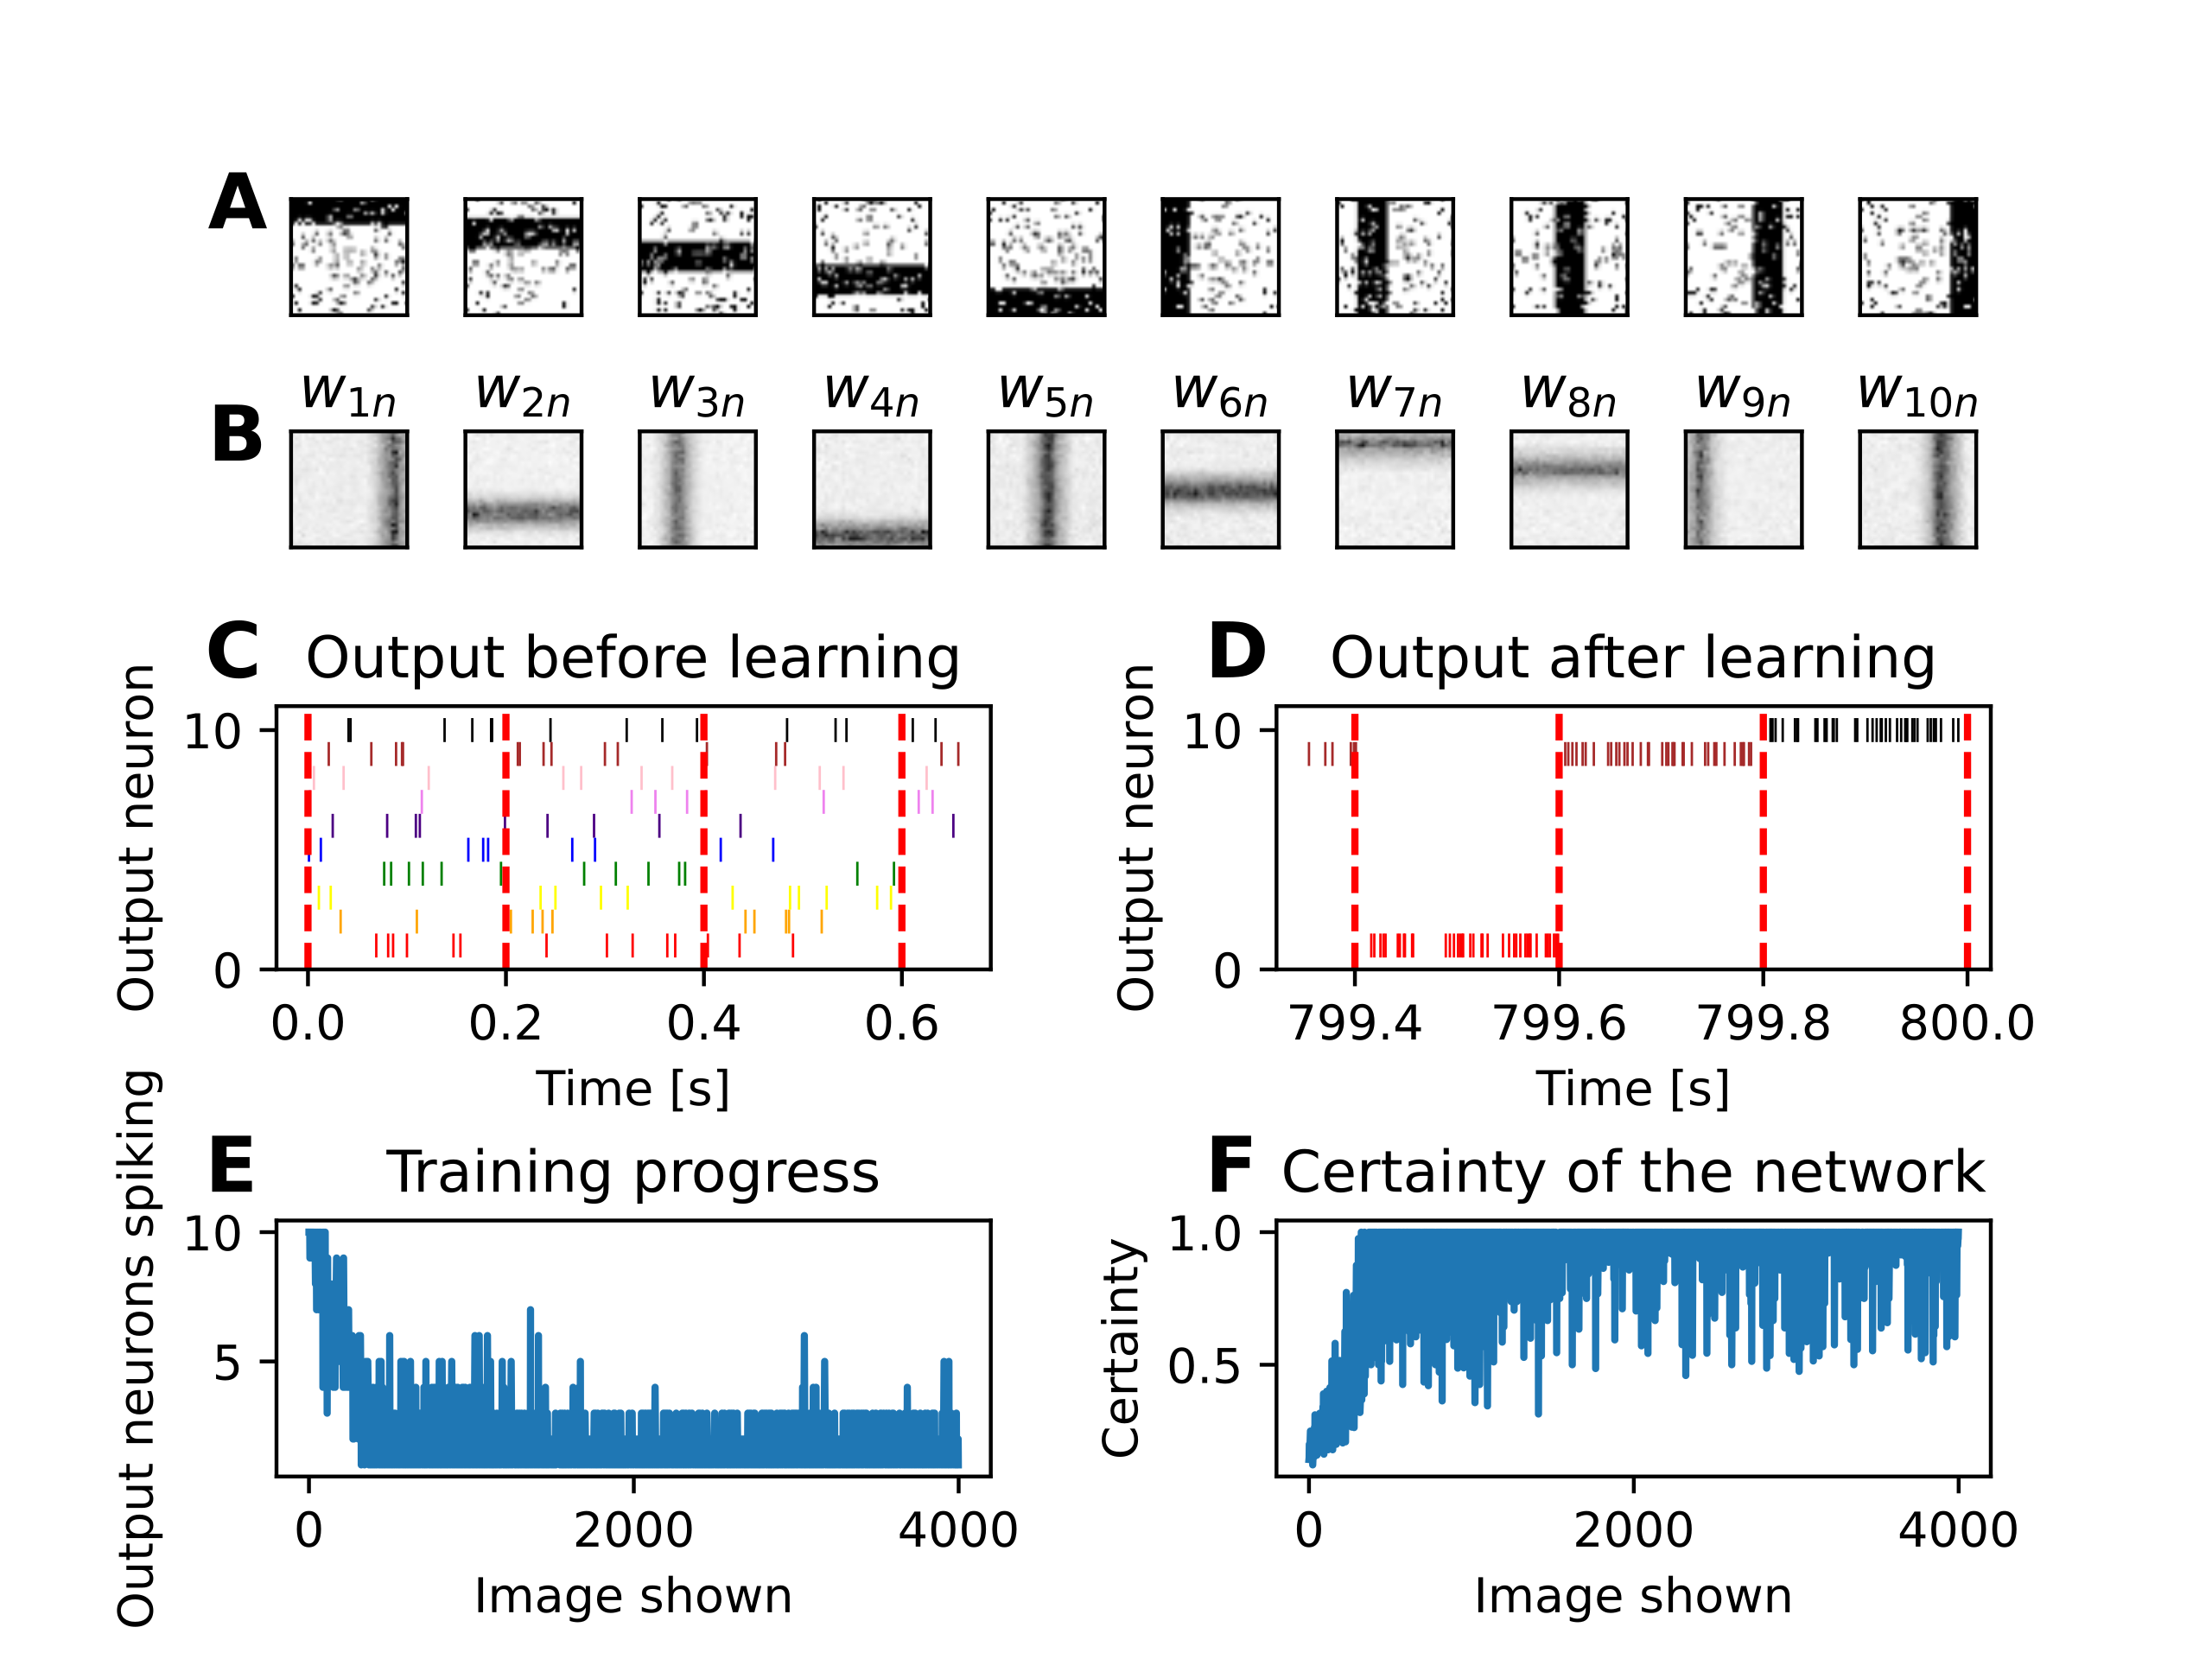
\includegraphics[width=\linewidth]{figures/horvertAdaptiveInh/trainingPlot.png}
  \caption{\textbf{Training with 20 prior neurons.} \textbf{A} Examples of 35 x 35-pixel input images of horizontal and vertical bars with background noise. \textbf{B} Learned weights of the connections between input and output neurons. \textbf{C, D} Spike activity expressed by the output neurons before and after the training of the network. \textbf{E} Number of distinct output neurons active during the presentation duration of each training image. \textbf{F} Proportion of most active output neuron  to activity of all other output neurons during the presentation duration of each training image.}
  \label{fig:horvertAdaptiveInhibitionTraining}
\end{figure}

\begin{figure}
  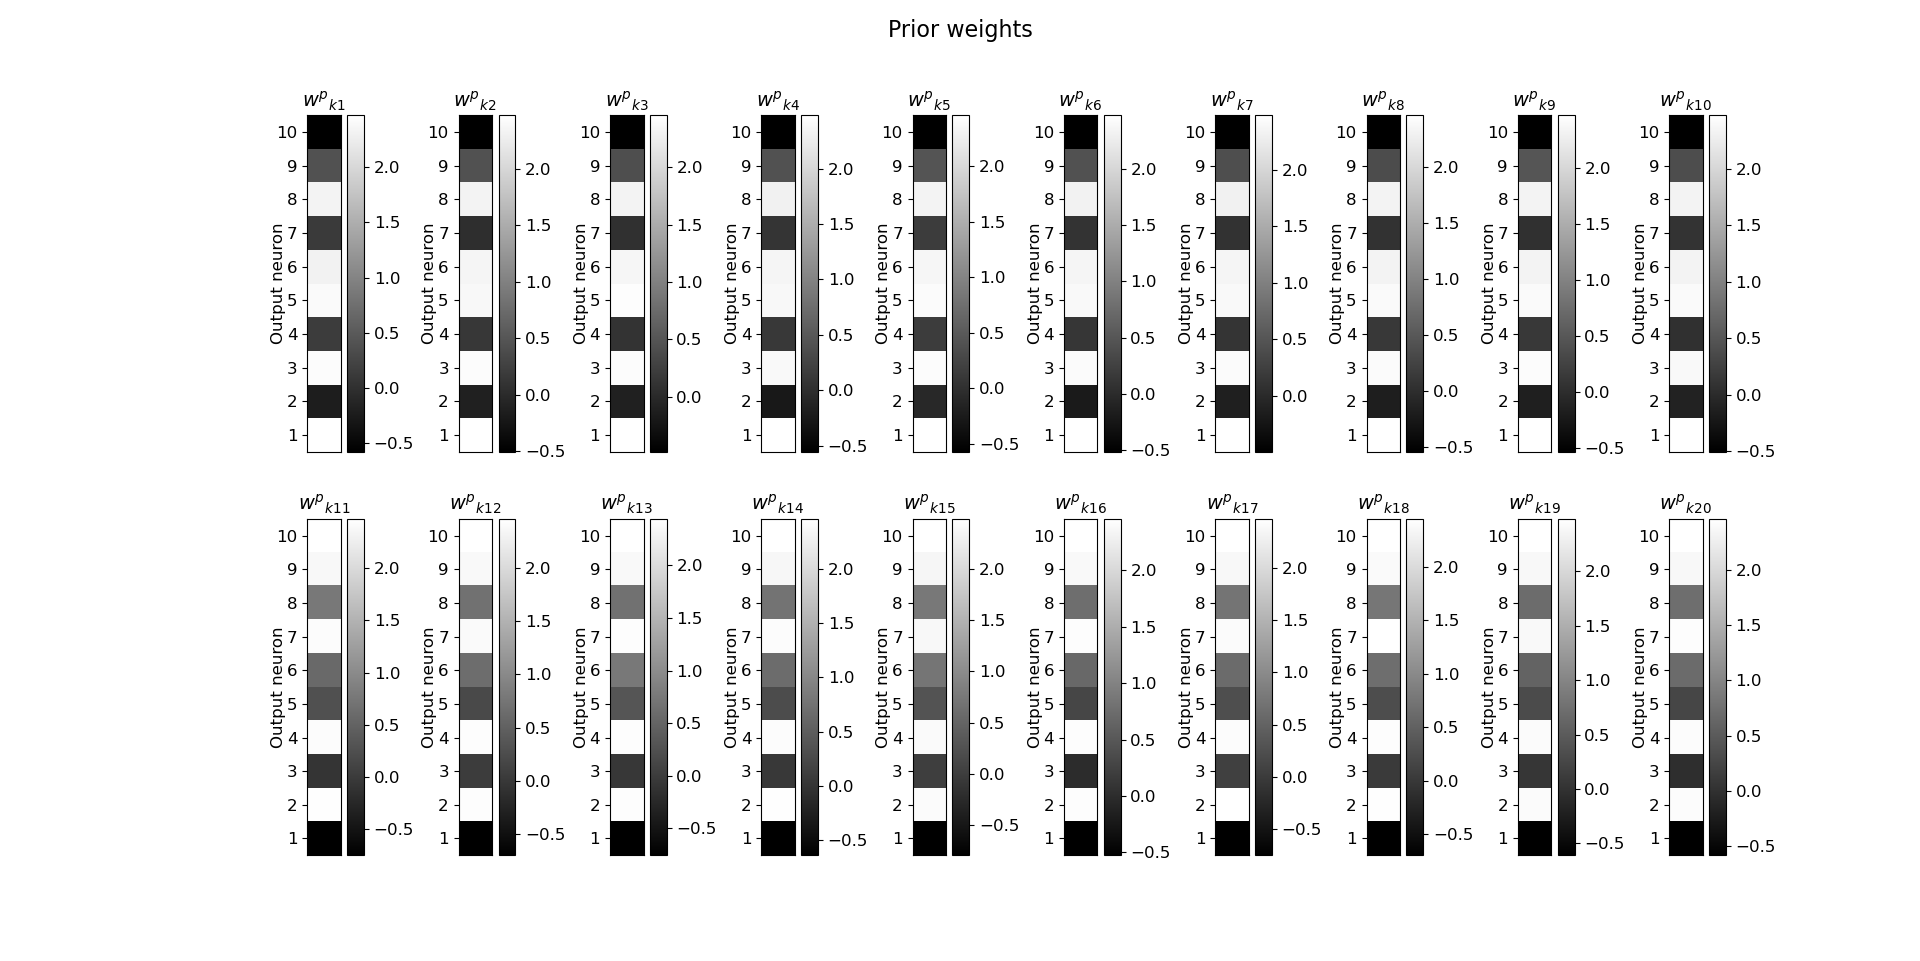
\includegraphics[width=\linewidth]{figures/horvertAdaptiveInh/priorWeights.png}
  \caption{ Learned weights of the connections between prior and output neurons. }
  \label{fig:horvertAdaptiveInhibitionpriorWeights}
\end{figure}

Next the impact of the prior was checked. To do this an image with one horizontal (at pixel 12) and one vertical bar (at pixel 5) on it was generated. Then the prior was set once to 0 (vertical) and once to 1 (horizontal). The image and the prior was then fed to the network. The cross image can be seen in Figure \ref{fig:horvertAdaptiveInhibitionPriorValImage}. The spiking activity depending on the prior can be seen in Figures \ref{fig:horvertAdaptiveInhibitionPriorValSpikes0} and \ref{fig:horvertAdaptiveInhibitionPriorValSpikes1}.

\begin{figure}
  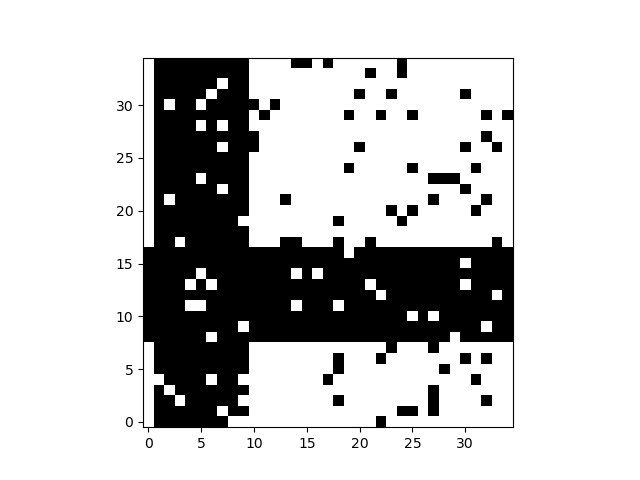
\includegraphics[width=\linewidth]{figures/horvertAdaptiveInh/20priors_pos5and12/crossImage.png}
  \caption{ Cross image fed to the network. }
  \label{fig:horvertAdaptiveInhibitionPriorValImage}
\end{figure}

\begin{figure}
  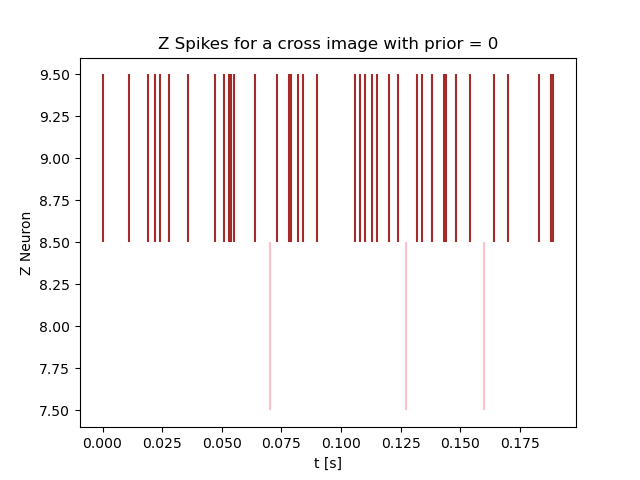
\includegraphics[width=\linewidth]{figures/horvertAdaptiveInh/20priors_pos5and12/crossZSpikes0.png}
  \caption{ Spiking activity of the output neurons with prior = 0. }
  \label{fig:horvertAdaptiveInhibitionPriorValSpikes0}
\end{figure}

\begin{figure}
  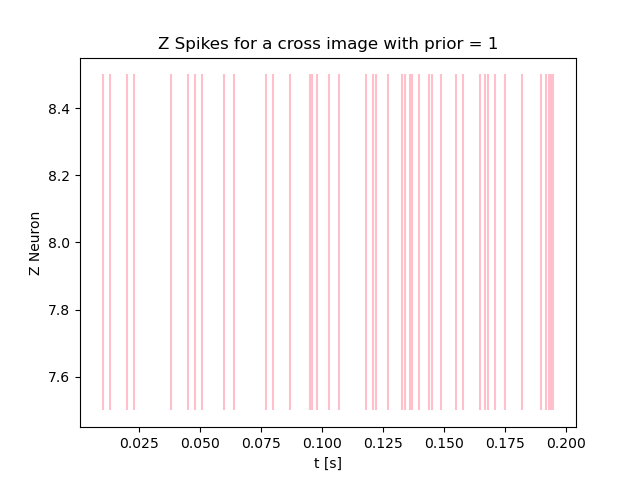
\includegraphics[width=\linewidth]{figures/horvertAdaptiveInh/20priors_pos5and12/crossZSpikes1.png}
  \caption{ Spiking activity of the output neurons with prior = 1. }
  \label{fig:horvertAdaptiveInhibitionPriorValSpikes1}
\end{figure}

To better show the impact of the prior it was gradually changed from horizontal to vertical. The starting firing frequency of the horizontal prior neurons was 200 Hz and 0 Hz for the vertical prior neurons. A cross image was shown to the network for 200 ms. After each image presentation duration the firing frequency of the horizontal prior neurons was decreased by 1 Hz and increased by 1 Hz for the vertical prior neurons. The used cross image can be seen in Figure \ref{fig:horvertAdaptiveInhibitionVariablePriorValImage}. The firing frequency of the 2 most active output neurons depending on the firing frequency of the vertical prior neurons can be seen in Figure \ref{fig:horvertAdaptiveInhibitionVariablePriorValFrequency}. As expected the correct horizontal output neuron is active in the beginning with about 200 Hz and the correct vertical output neuron is almost inactive. With rising firing frequency of the vertical prior neurons the activity of the horizontal output neurons decreases and the activity of the vertical output neurons increases. The membrane potentials of all output neurons for vertical prior neurons spiking with 200 Hz and horizontal prior neurons spiking with 0 Hz can be seen in Figure \ref{fig:horvertAdaptiveInhibitionVariablePriorValMembranePotentials}.

\begin{figure}
  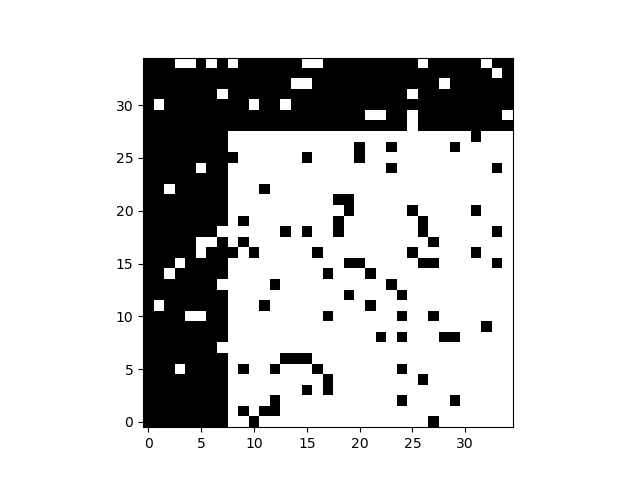
\includegraphics[width=\linewidth]{figures/horvertAdaptiveInh/crossImageForVariablePrior.png}
  \caption{ Cross image fed to the network. }
  \label{fig:horvertAdaptiveInhibitionVariablePriorValImage}
\end{figure}

\begin{figure}
  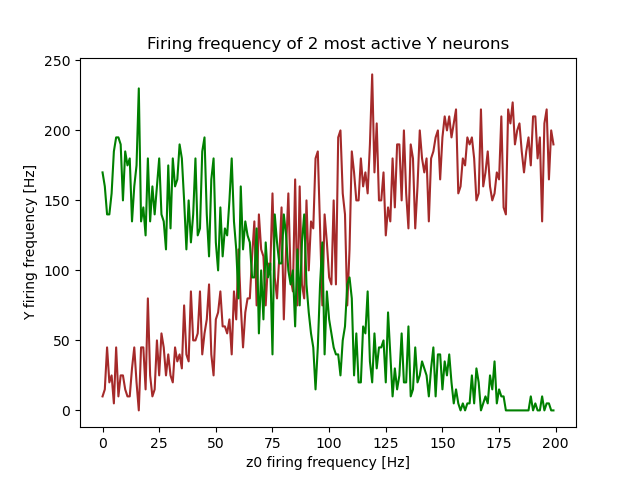
\includegraphics[width=\linewidth]{figures/horvertAdaptiveInh/YFrequency_prior199.png}
  \caption{ Firing frequency of the 2 most active output neurons depending on prior firing frequency. }
  \label{fig:horvertAdaptiveInhibitionVariablePriorValFrequency}
\end{figure}

\begin{figure}
  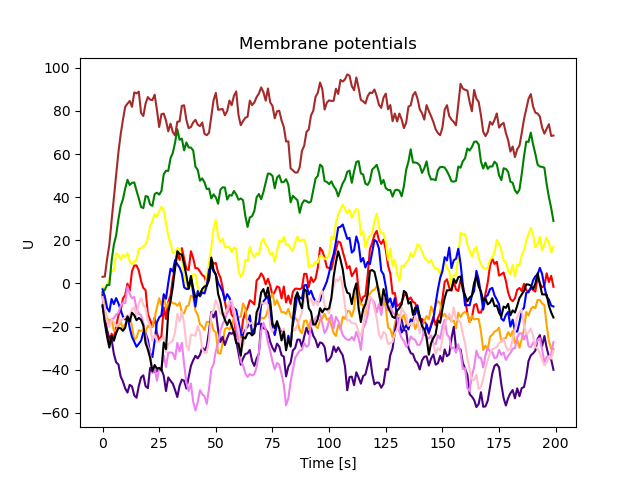
\includegraphics[width=\linewidth]{figures/horvertAdaptiveInh/membranePotentials0.png}
  \caption{ Membrane potentials of output neurons for vertical prior neurons spiking with 200 Hz and horizontal prior neurons spiking with 0 Hz. }
  \label{fig:horvertAdaptiveInhibitionVariablePriorValMembranePotentials}
\end{figure}








% unused exp, kept for looking up stuff

\iffalse
\section{Experiment 2: Horizontal and vertical bars}
\label{section:horvert}

 \subsection{Introduction}

For this experiment the impact of a neuron layer that encodes a-priori information should be analysed.

\subsection{Methods}

\paragraph{Input data}
29 x 29 black and white images with either horizontal or vertical oriented bars on them were used, as it was more straightforward to express a-priori information. The orientation of the training images was chosen randomly via a uniform distribution. Also the positions of the bars in the images were uniformly distributed. The rest of the image generation process is analogous to experiment 1, except no circular mask was used. Examples of the input data can be seen in Figure \ref{fig:horvertImages}. To show the value of the a-priori information validation images with two bars forming a cross were also generated, seen in Figure \ref{fig:horvertTrainingCrossImage}. When shown to the network in the validation process the prior neurons were given the information that a cross is either in horizontal or vertical orientation.

\begin{figure}
  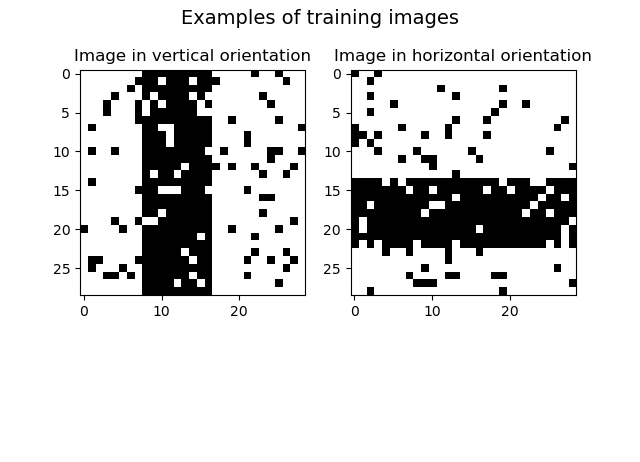
\includegraphics[width=\linewidth]{figures/horvert/horvertTrainingImages.png}
  \caption{Training images generated for experiment 2. One image of each possible orientation at a random position.}
  \label{fig:horvertImages}
\end{figure}

\begin{figure}
  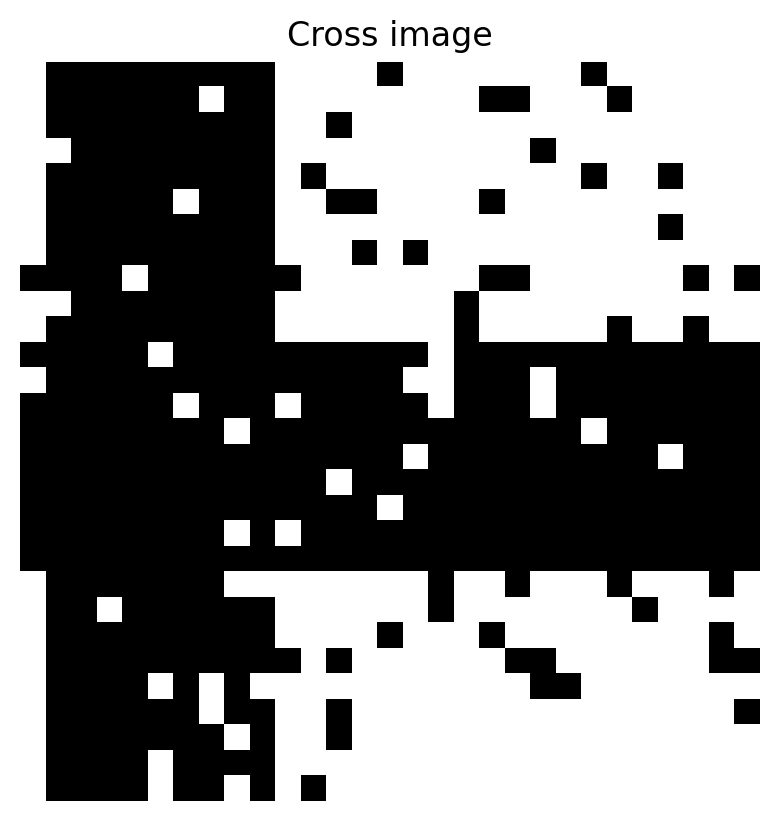
\includegraphics[width=0.6\linewidth]{figures/horvert/horvertTrainingCrossImage.png}
  \caption{Generated cross image which can represent either horizontal or vertical orientation.}
  \label{fig:horvertTrainingCrossImage}
\end{figure}


\paragraph{Network architecture}

This experiment used a expanded version of the network used in experiment 1. An additional layer of prior neurons $z_1,z_2$ was added. Whenever an image was oriented vertically $z_1$ was active and $z_2$ was inactive. For horizontal orientations $z_2$ was active and $z_1$ was inactive. Prior neurons in an active state had a firing frequency of 50 Hz and fired with 0 Hz when inactive.

\paragraph{Neuron model}
The input and output neurons functioned the same way as in the previous experiment. The prior neurons fire according to a poisson process with their firing rate. Each prior neuron $Z_l$ is connected to every output neuron $Y_k$ and thus has weights $w_{kl}$ that were learned by the network. 

\paragraph{Parameters}
As the amount of input neurons and the average number of black pixels in an input image stayed roughly the same in this experiment, the same parameters $c=  20$ and $\lambda = 10^{-3}$ could be used.

%% TODO START
%% this block was copied to Theoretical Background, cut this accordingly
%% Zfactor does not exist, remove!!!
 However as there are only two prior neurons, a way to amplify their produced signals was needed, otherwise their impact on the membrane potential of the output neurons would not be distinctive enough. So the EPSPs $z_l(t)$ were multiplied by the factor $Z_{factor}$. This factor was determined via grid search. The additional prior layer resulted in an expanded version of the membrane potential $u_k(t)$

\begin{equation}
\label{eqn:ukHorvert}
u_k(t) = \sum_{i=1}^n w_{ki} \cdot x_i(t) + \sum_{j=1}^n w_{kj} \cdot Z_{factor} \cdot z_j(t).
\end{equation}

%% TODO END

\subsection{Results} 

The following values for $Z_{factor} $ were tried with $c = 20$ and $\lambda = 10^{-3}$:
\begin{itemize}
  \item $Z_{factor} = 3$
  \item $Z_{factor} = 5$
  \item $Z_{factor} = 7$  
  \item $Z_{factor} = 10$ 
  \item $Z_{factor} = 20$
\end{itemize}

For $Z_{factor} = 10$ and $20$ the prior neurons impacted the learning progress negatively and let single prior neurons respond to too much area. An example of this can be seen in Figure \ref{fig:horvert_c20_3_Zfactor20_horizontalLines}

\begin{figure}
  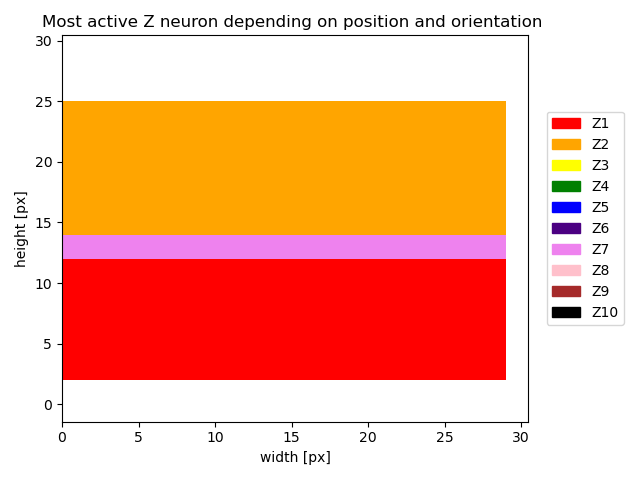
\includegraphics[width=\linewidth]{figures/horvert/horvert_c20_3_Zfactor20_horizontalLines.png}
  \caption{Most active output neuron for horizontal orientation and position on the y-axis of the training image during the training process. $c = 20, \lambda = 10^{-3}, Z_{factor} = 20$}
  \label{fig:horvert_c20_3_Zfactor20_horizontalLines}
\end{figure}


The best results were achieved with $Z_{factor} = 5$. When looking at the training progress in Figure \ref{fig:horvert_c20_3_Zfactor5_averageZ} it can be seen that the training accuracy is higher compared to experiment 1. This is due to the added a-priori information and the fact that less of each bar in an image is overlapping with multiple areas of output neurons. The network activity at the end of the training process can be seen in Figure \ref{fig:horvertLastSpikes}. In Figures \ref{fig:horvert_c20_3_Zfactor5_horizontalLines} and \ref{fig:horvert_c20_3_Zfactor5_verticalLines} the most active output neuron of the trained network is plotted for horizontal bars in every position and in the second plot for vertical bars in every position. Every one of the ten output neurons responds primarily to one coherent area in one orientation. The values of the learned prior weights $w_{kl}$ were plotted in Figures \ref{fig:wkl1} and \ref{fig:wkl2}. In these figures, in combination with Figures \ref{fig:horvert_c20_3_Zfactor5_horizontalLines} and \ref{fig:horvert_c20_3_Zfactor5_verticalLines}, can be seen that each prior neuron specialized on one orientation.

\begin{figure}
  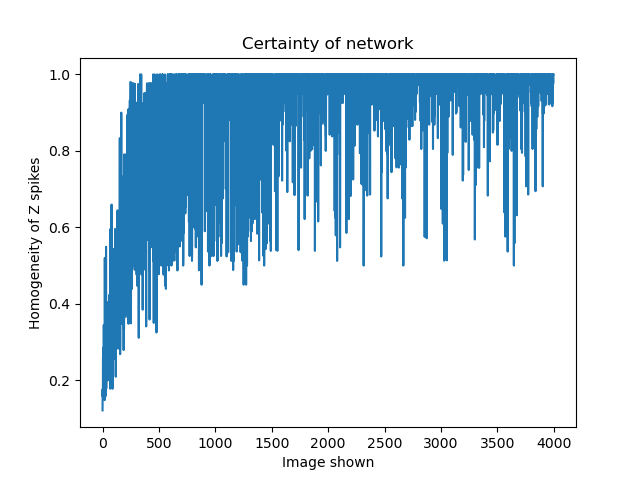
\includegraphics[width=\linewidth]{figures/horvert/horvert_c20_3_Zfactor5_averageZ.png}
  \caption{Proportion (accuracy) of most active output neuron  to activity of all other output neurons during the presentation duration of each training image. $c = 20, \lambda = 10^{-3}, Z_{factor} = 5$}
  \label{fig:horvert_c20_3_Zfactor5_averageZ}
\end{figure}

\begin{figure}
  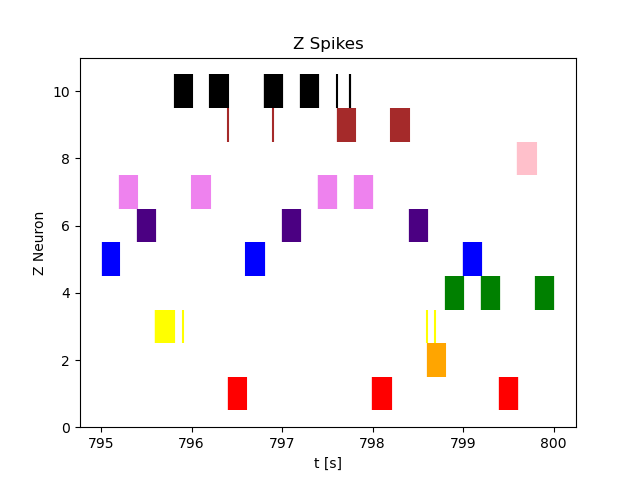
\includegraphics[width=\linewidth]{figures/horvert/horvert_c20_3_Zfactor5_1000LastZSpikes.png}
  \caption{Last 1000 output neuron spikes, $c = 20, \lambda = 10^{-3}$, $Z_{factor} = 5$}
  \label{fig:horvertLastSpikes}
\end{figure}

\begin{figure}
  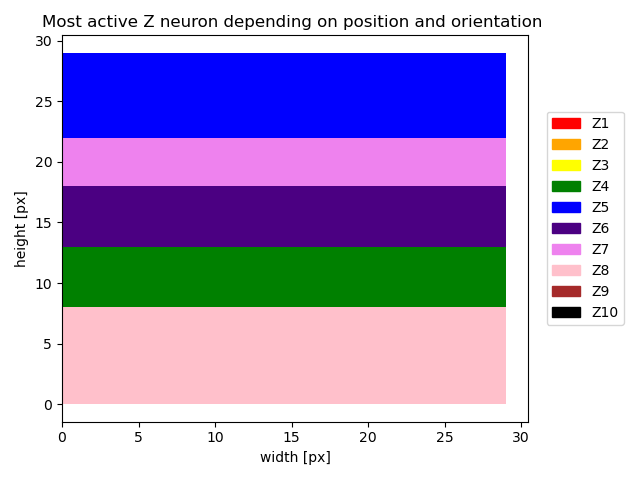
\includegraphics[width=\linewidth]{figures/horvert/horvert_c20_3_Zfactor5_horizontalLines.png}
  \caption{Most active output neuron for images of horizontal orientation and position on the x-axis of during the validation process. $c = 20, \lambda = 10^{-3}, Z_{factor} = 5$}
  \label{fig:horvert_c20_3_Zfactor5_horizontalLines}
\end{figure}

\begin{figure}
  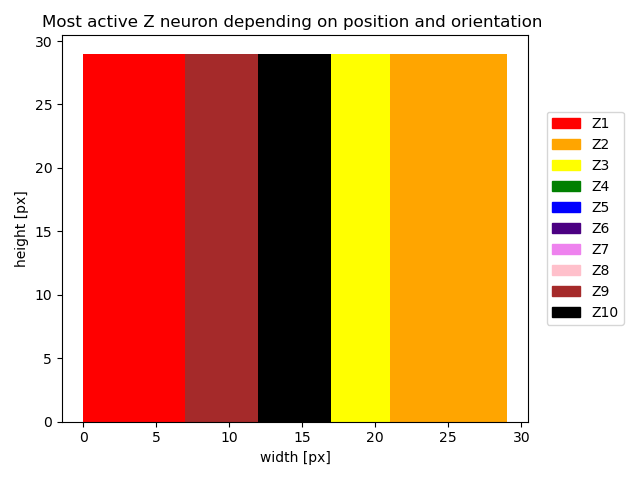
\includegraphics[width=\linewidth]{figures/horvert/horvert_c20_3_Zfactor5_verticalLines.png}
  \caption{Most active output neuron for images of vertical orientation and position on the x-axis of during the validation process. $c = 20, \lambda = 10^{-3}, Z_{factor} = 5$}
  \label{fig:horvert_c20_3_Zfactor5_verticalLines}
\end{figure}

\begin{figure}
  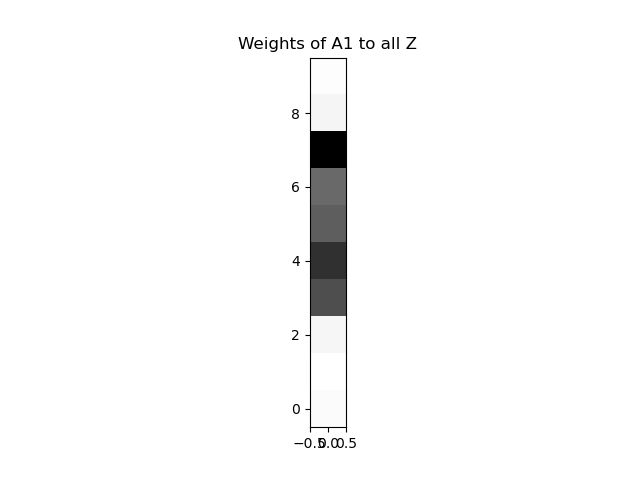
\includegraphics[width=\linewidth]{figures/horvert/horvert_c20_3_Zfactor5_priorWeight1.png}
  \caption{Values of $w_k1$, darker color means higher value. $c = 20, \lambda = 10^{-3}, Z_{factor} = 5$}
  \label{fig:wkl1}
\end{figure}

\begin{figure}
  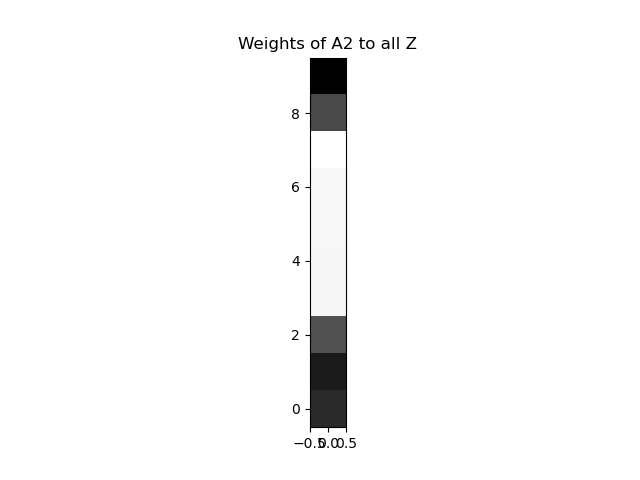
\includegraphics[width=\linewidth]{figures/horvert/horvert_c20_3_Zfactor5_priorWeight2.png}
  \caption{Values of $w_k2$, darker color means higher value. $c = 20, \lambda = 10^{-3}, Z_{factor} = 5$}
  \label{fig:wkl2}
\end{figure}

During the validation of all possible horizontal bar images the output spike activity was recorded and how many distinct output neurons were spiking during each image presentation period. For the parts where the 7 pixels high bar in the image did not overlap the areas of two output neurons only one output neuron was active. Only in the border areas there were two output neurons active. This can be seen in Figures \ref{fig:horvert_c20_3_Zfactor5_horizontalDistinctZ} and \ref{fig:horvert_c20_3_Zfactor5_horizontalZSpikes}. Compared to experiment 1 the activity is more homogeneous as each bar can only be in at most the area of four output neurons, when two of these areas are reinforced by the prior neurons.

\begin{figure}
  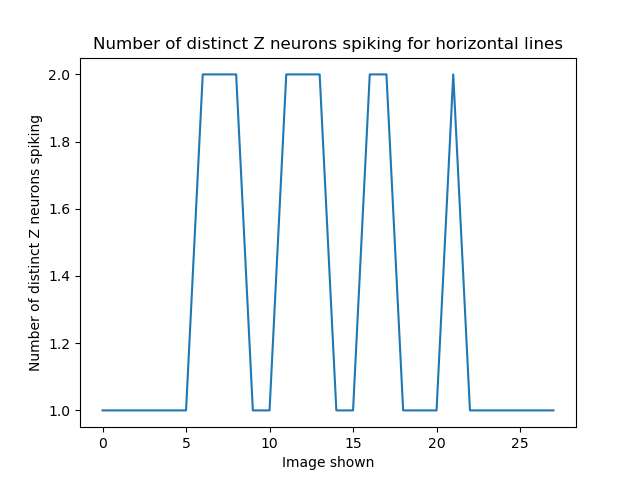
\includegraphics[width=\linewidth]{figures/horvert/horvert_c20_3_Zfactor5_horizontalDistinctZ.png}
  \caption{Distinct output neurons spiking during the presentation of all possible horizontal oriented validation images, $c = 20, \lambda = 10^{-3}$, $Z_{factor} = 5$}
  \label{fig:horvert_c20_3_Zfactor5_horizontalDistinctZ}
\end{figure}
\begin{figure}
  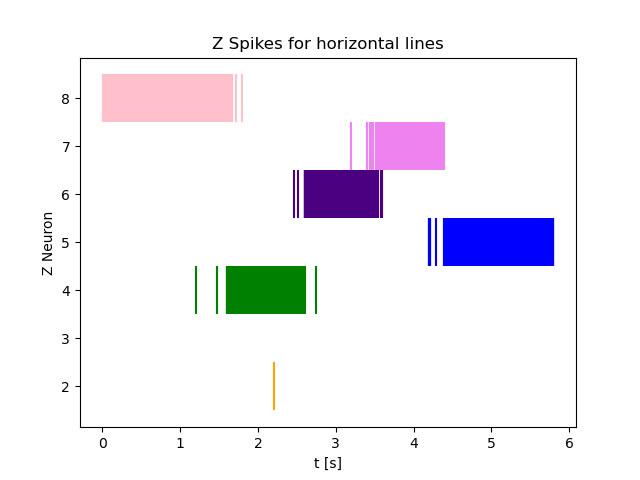
\includegraphics[width=\linewidth]{figures/horvert/horvert_c20_3_Zfactor5_horizontalZSpikes.png}
  \caption{Output neuron spikes during the presentation of all possible horizontal oriented validation images, $c = 20, \lambda = 10^{-3}$, $Z_{factor} = 5$}
  \label{fig:horvert_c20_3_Zfactor5_horizontalZSpikes}
\end{figure}


To show the impact of the prior neurons an image with two bars on it forming a cross (Figure \ref{fig:horvertValidationCross}) was generated and $z_2$ was set active indicating that the orientation is supposed to be horizontal. This resulted in the spiking pattern seen in Figure \ref{fig:horvert_c20_3_Zfactor5_crossZSpikes}. In it $Y_1$ is more active than $Y_9$ due to the influence of the prior neuron $Z_2$.

\begin{figure}
  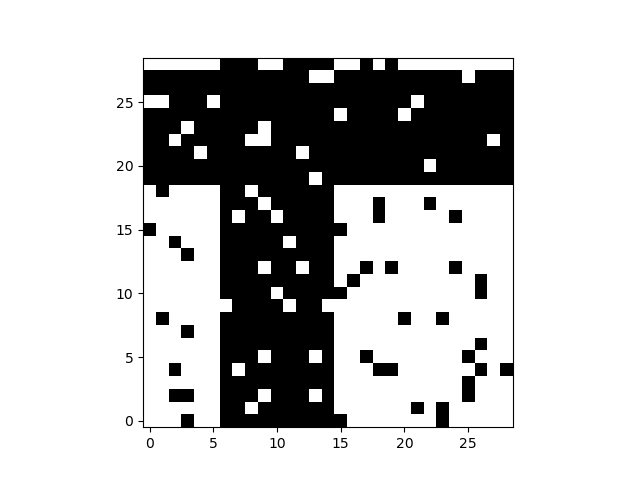
\includegraphics[width=\linewidth]{figures/horvert/horvert_c20_3_Zfactor5_validationCross.png}
  \caption{Generated validation cross image, with orientation defined as horizontal. $c = 20, \lambda = 10^{-3}, Z_{factor} = 5$}
  \label{fig:horvertValidationCross}
\end{figure}

\begin{figure}
  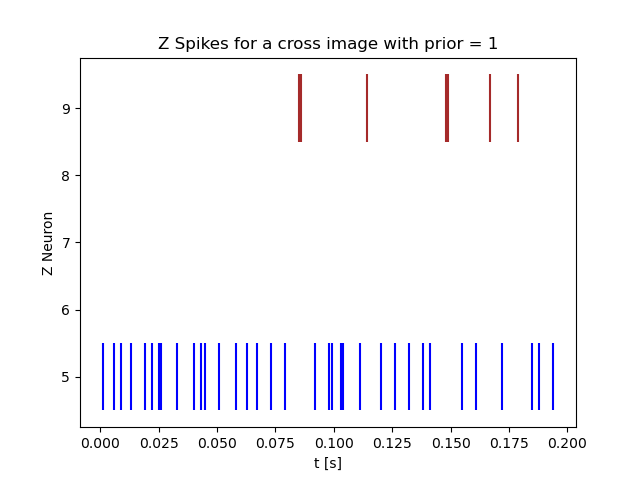
\includegraphics[width=\linewidth]{figures/horvert/horvert_c20_3_Zfactor5_crossZSpikes.png}
  \caption{Output spikes during the presentation of the validation cross image. $c = 20, \lambda = 10^{-3}, Z_{factor} = 5$}
  \label{fig:horvert_c20_3_Zfactor5_crossZSpikes}
\end{figure}

\fi